\section{Boundary element methods with Bempp}
In this section we want to provide a brief introduction to boundary element methods and describe the necessary steps for their numerical discretisation and solution.

The most simple boundary integral equation is of the form
\begin{equation}
	\label{eq:bnd_integral}
	\int_{\Gamma} g(\bx, \by)\phi(\by)ds(\by) = f(\bx),~\bx\in\Gamma.
\end{equation}
The function $g(\bx, \by)$ is a Green's function, $f$ is a given right-hand side and $\phi$ is an unknown surface density over the boundary $\Gamma$ of a bounded three dimensional domain $\Omega\subset\mathbb{R}^3$. To provide a concrete example. To compute the electrostatic capacity of an object $\Omega$ one solves the above equation with $f(\bx)$ the constant function $1$ and $g(\bx,\by)=\frac{1}{4\pi|\bx - \by|}$. The normalized capacity is then obtained as $c = \frac{1}{4\pi}\int_{\Gamma}\phi(\bx)ds(\bx)$. Many practical problems have a significantly more complex structure and can involve block systems of integral equations. Nevertheless, the fundamental structure of what Bempp-cl does is well described by the above problem and will be described in the following.

\begin{figure}
	\center
	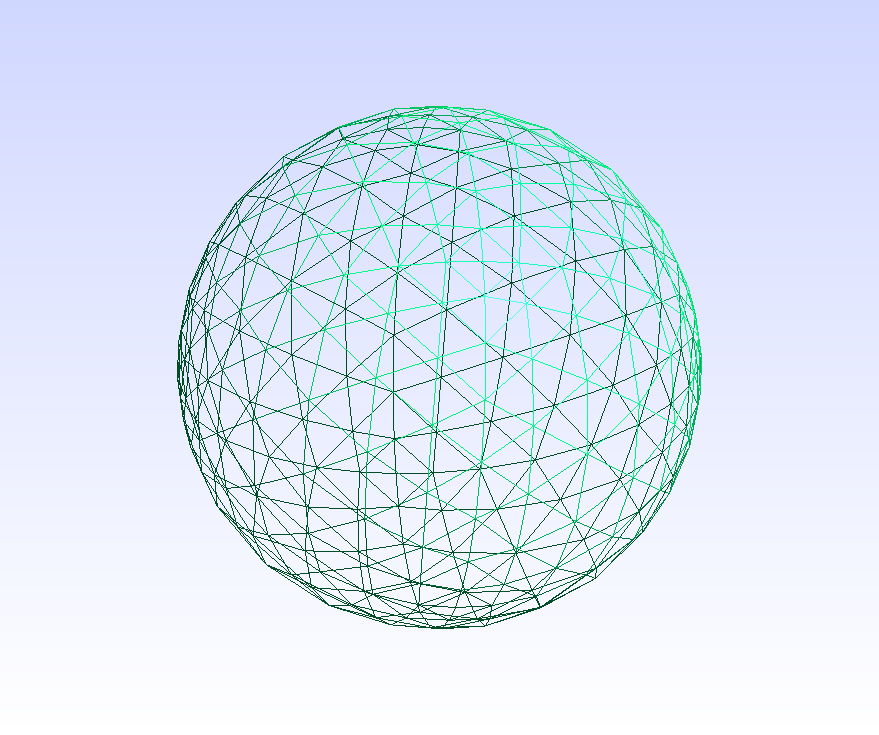
\includegraphics[width=5cm]{img/sphere}
	\label{fig:triangulation}
	\caption{Discretisation of a sphere into flat surface triangles.}
\end{figure}

The first step is the \textbf{definition of the surface} $\Gamma$. Surfaces are represented in Bempp-cl as a triangulation into flat triangles (see \ref{fig:triangulation}). The triangulation is internally represented as an array of node coordinates and an associated connectivity array of node indices that define each triangle. In this step also topology data is computed. In particular, for each triangle the neighboring triangles and the type of intersection (i.e. via joint node or edge) is computed.

Once a triangulation is given we need to define the necessary data structures for the discretisation. Bempp-cl uses a Galerkin discretisation. Consider \eqref{eq:bnd_integral}. We represent the solution $\phi$ as $\phi=\sum_{j=}^N x_j\phi_j$, where the $\phi_i$ are basis functions of a \textbf{trial space}, defined in the most simple case as constant $1$ on the triangle $\tau_j$ and $0$ everywhere also. Several other types of discretisation spaces are available in Bempp. Moreover, we require a \textbf{test (or dual) space} for the discretisation. Let $\psi=\sum_{i=1}^Ny_i \psi_i$, where each $\psi_i$ is a basis function of a space of test functions. For simplicity, here we will assume that the $\psi_i$ are also piecewise constant. The discrete representation of the above problem then takes the form

$$
Ax = b
$$
with 
$$
A_{ij} = \int_{\Gamma}\psi_i(\bx)\int_{\Gamma}g(\bx, \by)\phi_j(\bx)ds(\by)ds(\bx)
$$
and $f_i = \int_{\Gamma}\psi_i(\bx)f(\bx)ds(\bx)$. In the case of piecewise constant trial and test functions the definition of $A_{ij}$ simplifies to $A_{ij} = \int_{\Gamma}\int_{\Gamma}g(\bx, \by)ds(\by)ds(\bx)$.

In Bempp-cl an operator definition consists of the type of the operator (e.g. Laplace single-layer in the above example),
the definition of the trial and test spaces, and the definition of the range space. The range space is required for operator
products and not relevant for the purpose of this paper. The function $f$ is represented as a \textbf{Grid function object}, which
consists of either the dual representation in the forms of the integrals $b_i = \int_{\Gamma}\psi_i(\bx)f(\bx)ds(x)$ or directly through its coefficients $f_j$ in the representation $f=\sum_{j=1}^N f_j\phi_j$.

Once the grid, the space objects, and the operator are defined, the main computational step is performed, namely the \textbf{computation of the discrete matrix entries} $A_{ij}$. For pairs of triangles $\tau_i$ and $\tau_j$ that do not share a joint edge or vertex this is done through a simple numerical quadrature rule that approximates $A_{ij}\approx \sum_{\ell}\sum_{q} g(\bx_\ell, \by_q)\psi_i(\bx_\ell)\phi_j(\by_q)\omega_\ell\omega_q$, where the $\bx_\ell$ and $\by_q$ are quadrature points in the corresponding triangles $\tau_i$ and $\tau_j$, and the values $\omega_i$ and $\omega_j$ are the quadrature weights. In the case that two triangles share a joint vertex/edge or the triangles $\tau_i$ and $\tau_j$ are identical, corresponding singularity adapted quadrature numerical quadrature rules are used that are based on singularity removing coordinate transformations.

The values $b_i$ of the right-hand side vector $b$ are similarly computed through a numerical quadrature rule.

In the final step, \textbf{Bempp solves the underlying linear system of equations} either through a direct LU decomposition or through iterative solvers such as Gmres. The solution can then be evaluated away from the surface $\Gamma$ through domain potential operators and exported in various formats for visualization.

In summary, to solve a boundary integral equation problem, the following steps are performed by Bempp
\begin{enumerate}
	\item Import of the surface description as triangulation data
	\item Definition of the trial space, test space and range space
	\item Discretization into a matrix problem $Ax=b$
	\item Evaluation of domain potential operators for visualization and post-processing
\end{enumerate}

All of these steps are accelerated through the use of either Numba or OpenCL. In the following section we provide a high-level overview of the library and how these acceleration techniques are deployed before we deep dive into the design of the computational kernels.
